\chapter{Symulacja dynamiczna}\label{chap:dynamic}

W rzeczywistych sieciach społecznościowych wierzchołki i połączenia pojawiają się i znikają w czasie. Statyczny model dominowania nie oddaje tej dynamiki, dlatego w kolejnej serii badań wykorzystano symulator sieci dynamicznych. W takich warunkach algorytm powinien nie tylko znaleźć dobre rozwiązanie początkowe, lecz także utrzymywać niskie koszty w kolejnych krokach przy umiarkowanych nakładach czasowych.

\section{Założenia symulacji}

Każdą symulację rozpoczynano od bazowych grafów syntetycznych ($n\in\{20,40,80,160,320,640\}$) generowanych metodami \emph{random}, \emph{small\_world} i \emph{scale\_free}. Dla grafów syntetycznych rozważano trzy poziomy intensywności zmian (niski, średni, wysoki). Każdy poziom określają prawdopodobieństwa mutacji:

\begin{table}[H]
\centering
\begin{tabular}{|l|c|c|c|c|}
\hline
\textbf{Poziom intensywności} & \textbf{Dodawanie węzłów} & \textbf{Usuwanie węzłów} & \textbf{Dodawanie krawędzi} & \textbf{Usuwanie krawędzi} \\
\hline
\textbf{niski} & 0,02 & 0,01 & 0,06 & 0,04 \\
\textbf{średni} & 0,06 & 0,04 & 0,18 & 0,12 \\
\textbf{wysoki} & 0,12 & 0,08 & 0,30 & 0,20 \\
\hline
\end{tabular}
\caption{Parametry intensywności mutacji w symulacji dynamicznej.}
\label{tab:mutation_params}
\end{table}

Przy każdej mutacji węzły i krawędzie wybierano losowo. Symulację uruchamiano na 30 kroków; w każdym kroku stosowano jedną realizację mutacji. Po każdej modyfikacji sieci uruchamiano wszystkie algorytmy z tabeli \ref{tab:algorithms} (rozdział \ref{chap:experiments}) dla dwóch konfiguracji licencyjnych (\emph{duolingo\_super}, \emph{roman\_domination}). Ze względu na czas obliczeń analizę ograniczono do 45 s na krok.

Wersja \emph{dynamic\_real} odwzorowuje bardziej realistyczne ewolucje sieci, korzystając z funkcji preferencyjnego przyłączania i motywu triadycznego; do tej serii wygenerowano warianty \emph{pref\_triadic}, \emph{pref\_pref} oraz \emph{rand\_rewire} dla grafów o rozmiarach 40--640 węzłów.

\textbf{Uwaga:} Dalsza część rozdziału opiera się na już dostępnych wynikach dla wariantu o \textbf{niskiej intensywności} (\emph{dynamic\_low}); wyniki dla wariantów średnich, wysokich oraz realistycznych zostaną uzupełnione w finalnej wersji pracy po zakończeniu obliczeń.

\section{Zbiór danych i filtracja}

Wariant \emph{dynamic\_low} wygenerował 8\,262 pomiarów; po ograniczeniu do licencji \emph{duolingo\_super}, prawidłowych rozwiązań (\texttt{valid=True}) i usunięciu timeoutów pozostało 4\,005 obserwacji. Każda obserwacja zawierała: krok symulacji \texttt{step}, liczbę węzłów \texttt{n\_nodes}, koszt \texttt{total\_cost}, czas wykonania \texttt{time\_ms}, rozmiary grup licencyjnych oraz wskaźnik, czy algorytm korzystał z \emph{warm startu}. Dodatkowo obliczono koszt w przeliczeniu na węzeł \texttt{cost\_per\_node}, aby umożliwić porównania między grafami o różnej wielkości.

\section{Ewolucja kosztu i czasu -- niski poziom intensywności}

Rysunki \ref{fig:er_cost_step}--\ref{fig:ba_time_step} prezentują średni \textbf{koszt na wierzchołek} oraz \textbf{czas wykonania} w funkcji kroku symulacji dla poszczególnych klas grafów. Linie są średnią z wszystkich rozmiarów początkowych dla danej klasy grafu i algorytmu; osie Y są przedstawione w skali liniowej (koszt) i logarytmicznej (czas).

\subsection{Grafy losowe (ER)}

Koszt na wierzchołek stopniowo rośnie wraz ze wzrostem liczby kroków dla wszystkich algorytmów, jednak metaheurystyki (GA, SA, TS, ACO) zachowują przewagę nad heurystykami \textbf{GreedyAlgorithm} i baseline'em \textbf{RandomizedAlgorithm}. Czas wykonania dla metaheurystyk systematycznie rośnie (wykładniczo na skali liniowej), podczas gdy \textbf{GreedyAlgorithm} i \textbf{RandomizedAlgorithm} pozostają blisko 1--10 ms niezależnie od kroku.

\begin{figure}[H]
  \centering
  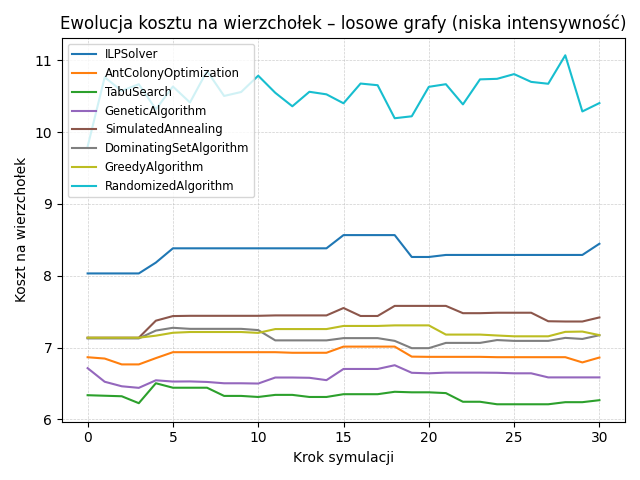
\includegraphics[width=0.48\linewidth]{assets/figures/er_cost_vs_step.png}
  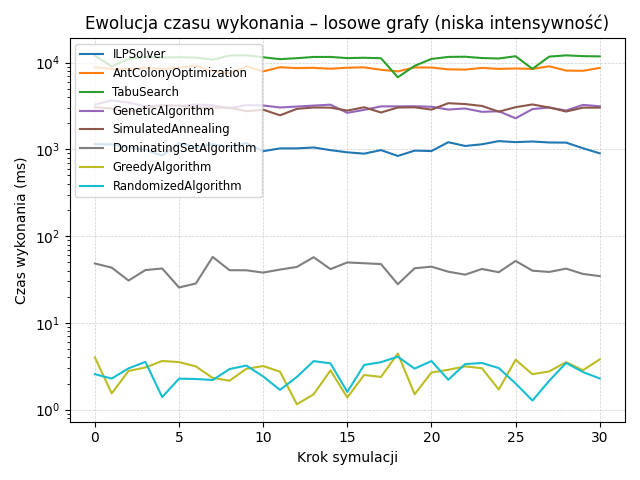
\includegraphics[width=0.48\linewidth]{assets/figures/er_time_vs_step.png}
  \caption{Grafy ER: koszt na węzeł i czas wykonania vs krok symulacji.}
  \label{fig:er_cost_step}
\end{figure}

\subsection{Grafy małoświatowe (WS)}

Początkowy koszt jest nieco niższy niż w grafach losowych; metaheurystyki nieco szybciej stabilizują się, a heurystyki \textbf{GreedyAlgorithm}/\textbf{DominatingSetAlgorithm} pozostają bardziej konkurencyjne. Czas ACO, TS i GA jest wciąż wysoki, ale rośnie wolniej niż w ER.

\begin{figure}[H]
  \centering
  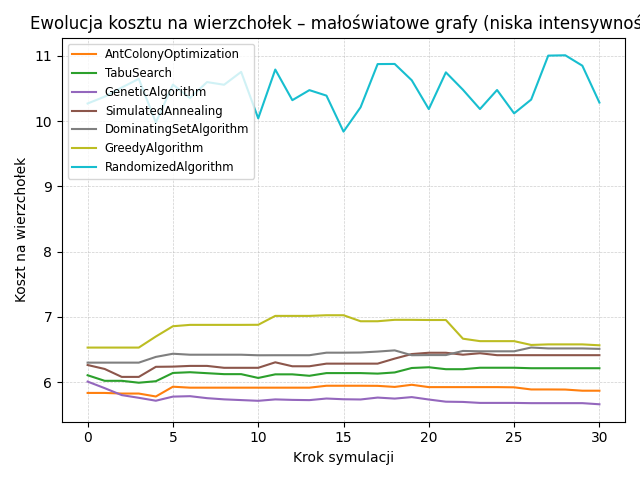
\includegraphics[width=0.48\linewidth]{assets/figures/ws_cost_vs_step.png}
  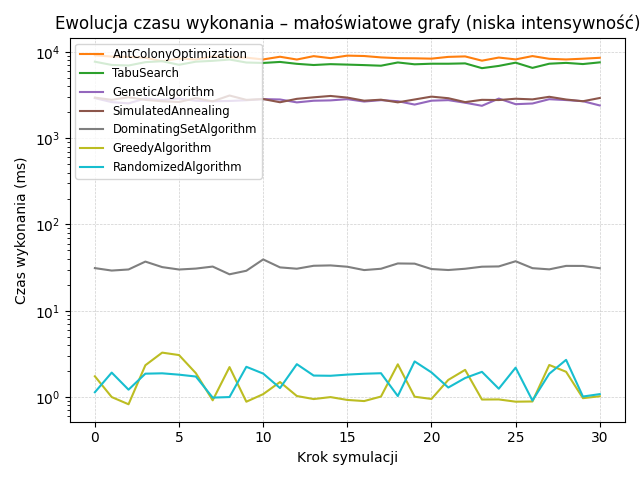
\includegraphics[width=0.48\linewidth]{assets/figures/ws_time_vs_step.png}
  \caption{Grafy WS: koszt na węzeł i czas wykonania vs krok symulacji.}
  \label{fig:ws_cost_step}
\end{figure}

\subsection{Grafy bezskalowe (BA)}

Dzięki obecności hubów koszty metaheurystyk utrzymują się na niskim poziomie nawet w późnych krokach; \textbf{GreedyAlgorithm} nadal jest najlepszy z prostych heurystyk (z wyjątkiem baseline'u \textbf{RandomizedAlgorithm}). Czas ACO jest największy, ale rośnie nieznacznie wolniej niż w ER.

\begin{figure}[H]
  \centering
  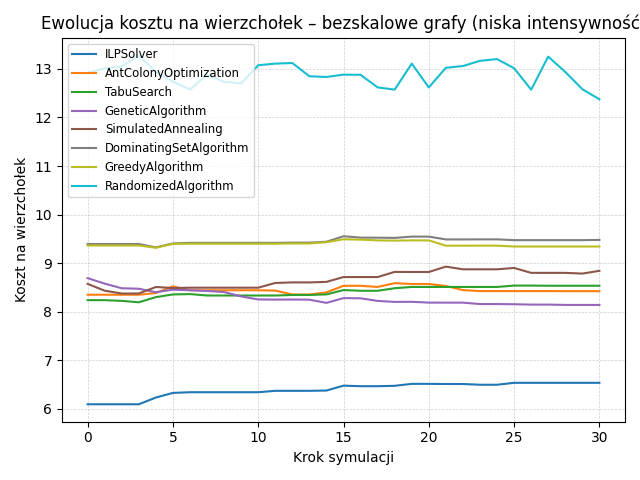
\includegraphics[width=0.48\linewidth]{assets/figures/ba_cost_vs_step.png}
  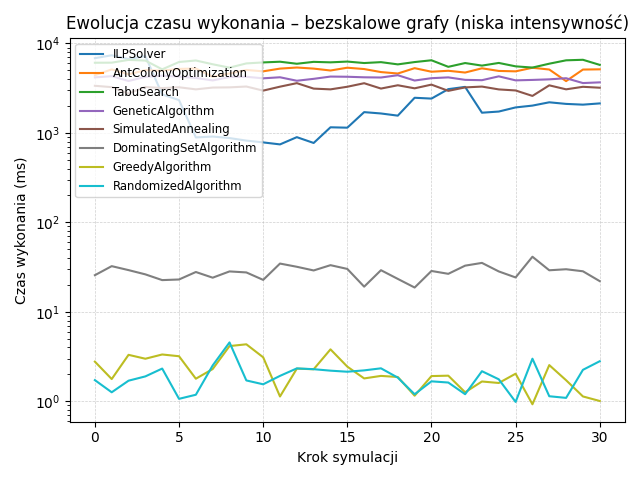
\includegraphics[width=0.48\linewidth]{assets/figures/ba_time_vs_step.png}
  \caption{Grafy BA: koszt na węzeł i czas wykonania vs krok symulacji.}
  \label{fig:ba_time_step}
\end{figure}

\section{Ranking algorytmów w ostatnim kroku}

W tabeli \ref{tab:dynamic_final_step} zestawiono średni koszt na węzeł i czas wykonania w \textbf{ostatnim} kroku symulacji (krok 30) dla wariantu niskiej intensywności. Ostatni krok reprezentuje stan sieci po 30 mutacjach.

\begin{table}[H]
\centering
\begin{tabular}{|l|r|r|r|}
\hline
\textbf{Algorytm} & \textbf{Liczba obserwacji} & \textbf{Średni koszt na wierzchołek} & \textbf{Średni czas (ms)} \\
\hline
\textbf{GreedyAlgorithm} & 18 & 7,7 & 2 \\
\textbf{DominatingSetAlgorithm} & 18 & 7,7 & 29 \\
\textbf{GeneticAlgorithm} & 18 & 6,8 & 3070 \\
\textbf{SimulatedAnnealing} & 18 & 7,6 & 3050 \\
\textbf{AntColonyOptimization} & 14 & 7,0 & 7624 \\
\textbf{TabuSearch} & 18 & 7,0 & 8372 \\
\textbf{ILPSolver} & 7 & 7,1 & 1783 \\
\textbf{RandomizedAlgorithm} & 18 & 11,0 & 2 \\
\hline
\end{tabular}
\caption{Wydajność algorytmów w ostatnim kroku symulacji (krok 30).}
\label{tab:dynamic_final_step}
\end{table}

Algorytmy \textbf{GreedyAlgorithm} i \textbf{DominatingSetAlgorithm} pozostają bezkonkurencyjne pod względem szybkości, uzyskując koszt na wierzchołek zbliżony do metaheurystyk i \textbf{ILPSolvera}. Metaheurystyki (GA, SA, TS, ACO) minimalnie obniżają koszt w stosunku do heurystyk, lecz ich czasy są o rząd wielkości dłuższe. \textbf{ILPSolver} działa szybciej niż w scenariuszu statycznym dzięki mniejszym krokom symulacji, jednak nie zachowuje przewagi jakościowej. Baseline \textbf{RandomizedAlgorithm} potwierdza skuteczność wszystkich pozostałych metod.

\begin{figure}[H]
  \centering
  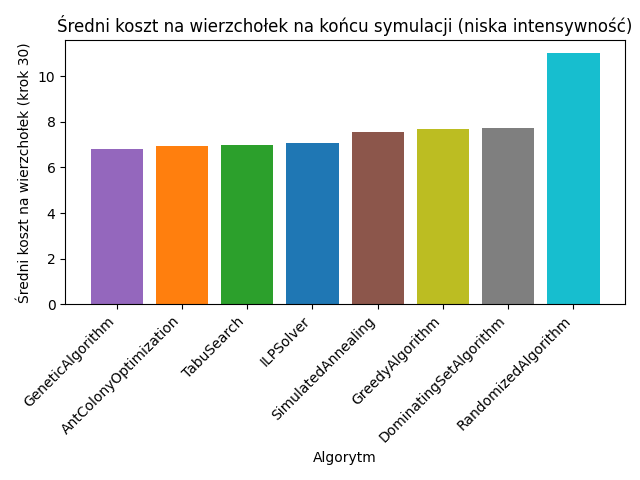
\includegraphics[width=0.48\linewidth]{assets/figures/final_step_cost.png}
  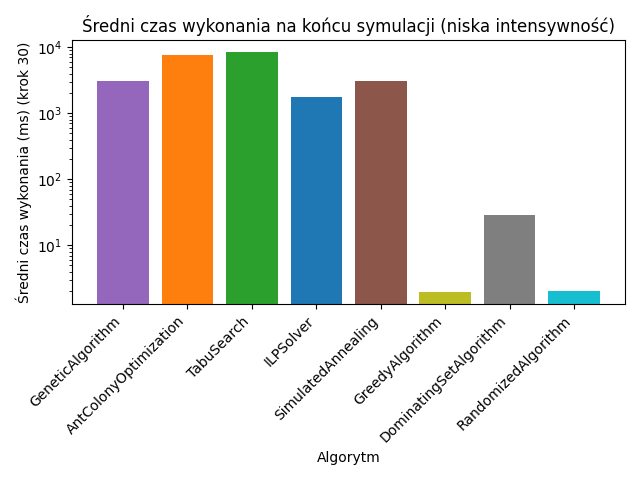
\includegraphics[width=0.48\linewidth]{assets/figures/final_step_time.png}
  \caption{Średni koszt na wierzchołek i czas wykonania na końcu symulacji.}
  \label{fig:dynamic_final_bars}
\end{figure}

\section{Wnioski z wariantu niskiej intensywności}

\begin{enumerate}
\item \textbf{Stabilność heurystyk} -- \textbf{GreedyAlgorithm} i \textbf{DominatingSetAlgorithm} utrzymują stabilny koszt i są niezwykle szybkie. Są więc rekomendowane w dynamicznym środowisku, w którym koszt obliczeń jest kluczowy.

\item \textbf{Metaheurystyki} -- ACO, TabuSearch, GA i SA oferują jedynie marginalne obniżenie kosztu w porównaniu do prostych heurystyk, lecz wymagają znacznie więcej czasu. Dla dynamicznych sieci ich zastosowanie jest uzasadnione jedynie, gdy priorytetem jest minimalizacja kosztów, a zasoby obliczeniowe nie są ograniczone.

\item \textbf{ILPSolver} -- w dynamicznej symulacji odnotowuje się krótszy czas pracy niż w przypadku statycznym, ale traci on przewagę jakościową; nie ma już znaczącej różnicy między ILP a metaheurystykami.

\item \textbf{Struktura grafu} -- grafy bezskalowe (BA) pozwalają utrzymać niższe koszty nawet przy dynamice sieci, co potwierdza wcześniejsze obserwacje dotyczące obecności węzłów o wysokim stopniu. Grafy losowe (ER) i małoświatowe (WS) wykazują większą wrażliwość na mutacje.

\item \textbf{Baseline} -- \textbf{RandomizedAlgorithm} potwierdza skuteczność wszystkich badanych algorytmów, osiągając znacznie wyższe koszty od pozostałych metod.
\end{enumerate}

\section{Ewolucja kosztu i czasu -- średni poziom intensywności}

\emph{TODO: wyniki dla dynamic\_medium}

\section{Ewolucja kosztu i czasu -- wysoki poziom intensywności}

\emph{TODO: wyniki dla dynamic\_high}

\section{Symulacje realistyczne -- preferencyjne dołączanie i triady}

\subsection{Wariant pref\_triadic}

\emph{TODO: wyniki dla pref\_triadic}

\subsection{Wariant pref\_pref}

\emph{TODO: wyniki dla pref\_pref}

\subsection{Wariant rand\_rewire}

\emph{TODO: wyniki dla rand\_rewire}

\section{Analiza warm start vs cold start}

\emph{TODO: porównanie warm vs cold dla wszystkich wariantów}



